\documentclass[border=5pt]{standalone}
\usepackage{pgfplots}
\pgfplotsset{compat=1.18}
\begin{document}
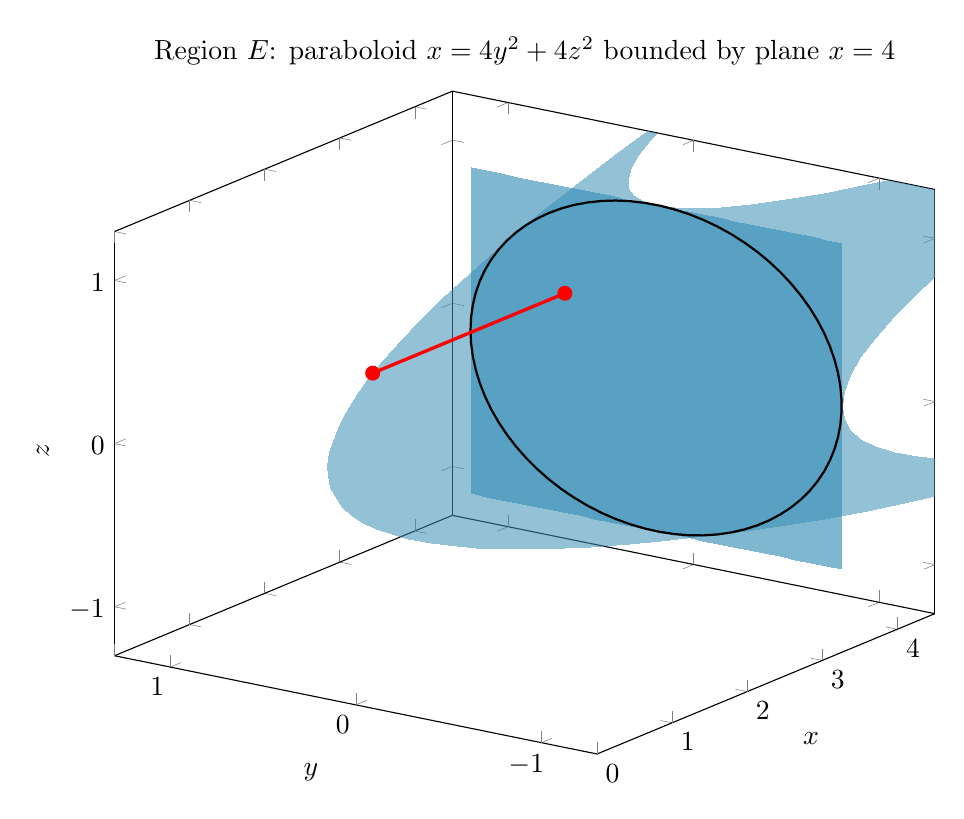
\begin{tikzpicture}
\begin{axis}[
    view={-55}{22},
    xlabel=$x$, ylabel=$y$, zlabel=$z$,
    xmin=0, xmax=4.5, ymin=-1.3, ymax=1.3, zmin=-1.3, zmax=1.3,
    xtick={0,1,2,3,4}, ytick={-1,0,1}, ztick={-1,0,1},
    title={Region $E$: paraboloid $x=4y^2+4z^2$ bounded by plane $x=4$},
    width=12cm, height=10cm,
    colormap={}{rgb=(0.227,0.561,0.718); rgb=(0.227,0.561,0.718)}
]
% Paraboloid x = 4y^2 + 4z^2, with y,z in [-1,1]
\addplot3[
    surf, shader=interp, samples=25, domain=-1:1, y domain=-1:1,
    opacity=0.55, fill opacity=0.55, draw=none,
] ({4*x^2 + 4*y^2}, {x}, {y});

% Plane x = 4 (disk y^2+z^2 <= 1)
\addplot3[
    surf, shader=interp, samples=25, domain=-1:1, y domain=-1:1,
    opacity=0.65, fill opacity=0.65, draw=none,
] (4, {x}, {y});

% Rim of disk at x=4
\addplot3[black, thick, samples=80, domain=0:2*pi, variable=\t]
    (4, {cos(deg(\t))}, {sin(deg(\t))});

% A sample vertical line segment inside E
\addplot3[red, very thick, samples=2, domain=0:1]
    ({4*(0.6*cos(35))^2 + 4*(0.6*sin(35))^2 + (4 - 4*(0.6*cos(35))^2 - 4*(0.6*sin(35))^2)*x},
     {0.6*cos(35)}, {0.6*sin(35)});
\addplot3[red, only marks, mark=*, mark size=2.5]
    coordinates {({4*(0.6*cos(35))^2 + 4*(0.6*sin(35))^2}, {0.6*cos(35)}, {0.6*sin(35)})
                 (4, {0.6*cos(35)}, {0.6*sin(35)})};
\end{axis}
\end{tikzpicture}
\end{document}